
\chapter{Measurement of Planck's Constant}

\section{Introduction}

In this lab, we will measure Planck's constant by measuring the
$V$-$I$ curves of three different colored light emitting diodes
(LEDs).  An LED is a particular type of diode for which the
recombination of electrons and holes produces photons, typically in
the visible light spectrum.  These diodes have an activation voltage given by:
\begin{equation} \label{eqn:va}
V_{\rm A} = \phi + \frac{hc}{e}\frac{1}{\lambda}
\end{equation}
where $\lambda$ is the wave-length of the light produced by the diode,
and $\phi$ is the contribution to the voltage drop due to other
effects in the $p-n$ junctions.  The diodes we are using have been
chosen to ensure that $\phi$ is approximately constant across all
three diodes.

The quantity
\begin{displaymath}
\frac{hc}{e}
\end{displaymath}
can therefore be determine from the slope of the activation voltage as a function of $1/\lambda$.

The 2018 redefinition of the SI is means that the quantity
\begin{displaymath}
hc = 1.23984193~\rm eV \mu m
\end{displaymath}
is technically now exactly known, because the values $h$, $c$, and $e$
are now taken as exact values which define the corresponding SI
units. Of course, it is still useful and fun to measure this quantity
ourselves in the lab.  Since we will also be measuring the speed of
light, we'll interpret this measurement as our determination of
Planck's constant.

\section{LED Model}

For the purpose of this experiment, we will model the LED as an ideal
diode with voltage drop equal to the activation voltage $V_{\rm A}$ of
Equation~\ref{eqn:va} plus a series resistance $R_{\rm LED}$.  As
shown in Fig.~\ref{fig:ledmodel}, the effect of this resistance is to
replace the vertical line at the activation voltage $V_A$ with a line
of slope $1/R_{\rm LED}$.

\begin{figure}[htbp]
\begin{center}
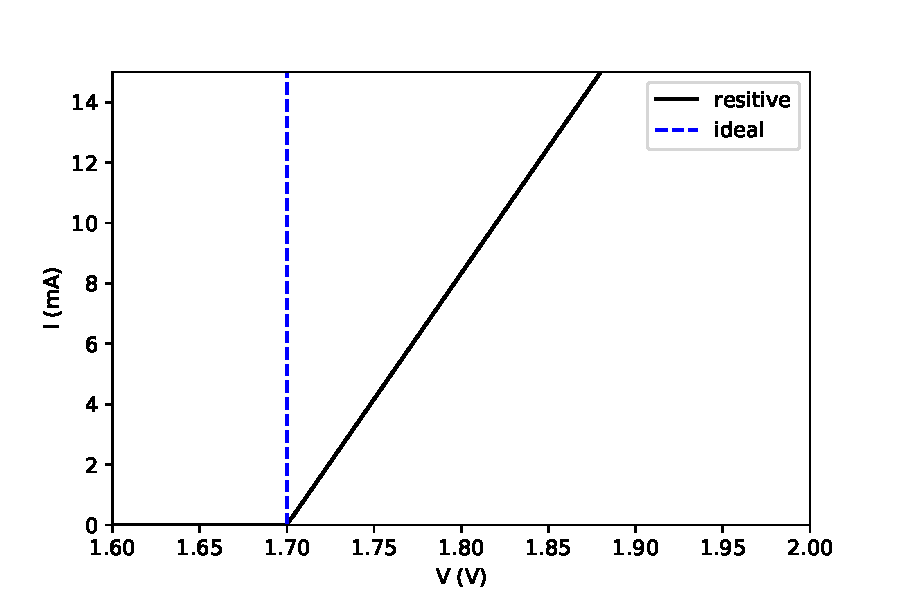
\includegraphics[height=0.3\textheight]{figs/labs/planck/model.pdf} \\
\end{center}
\caption{The LED model for $V_A=1.7~\rm V$ and $R_{\rm LED}=12~\Omega$}
\label{fig:ledmodel}
\end{figure}



\section{$V-I$ Curve from LED.}

\begin{figure}[htbp]
\begin{center}
\begin{circuitikz}[line width=1pt]
\draw (0,0) to[voltage source,bipoles/length=1.5cm,l=$V_1$] ++(0,4.0) to[short] ++(2.0,0) coordinate(C);
\draw (C) to[R, l_=$R_1$] ++(0,-2.0) coordinate(B) to[empty diode, l_=LED] ++(0,-2.0) coordinate(A) to[short] ++(-2.0,0.0);
\draw (A) to[short,*-] ++(1.5,0) to[short] ++(0,0.8) node[component]{V} to[short] ++(0,0.8) to[short,-*] ++(-1.5,0);
\draw (C) to[short,*-] ++(1.5,0) to[short] ++(0,-0.8) node[component]{V} to[short] ++(0,-0.8) to[short,-*] ++(-1.5,0);
\end{circuitikz} 
\end{center}
\caption{experimental setup.}
\label{fig:planck_setup}
\end{figure}

Construct the experimental setup shown in Fig.~\ref{fig:planck_setup}
using a $1~\rm k\Omega$ precision $1\%$ resistor for $R_1$, a green
LED (see Table~\ref{tbl:led}) , and using your bench-top DC supply to provide $V_1$, initially
set to $0~\rm V$.  Connect Mastech voltmeter across the resistor $R_1$ and
Triplett voltmeter across the LED.  When constructing your circuit,
make sure the LED can be easily removed and replaced.  Also keep in
mind that the longer lead is the positive terminal of the LED, i.e.,
the upper terminal of the LED as drawn in the
Fig.~\ref{fig:planck_setup}.  Set both voltmeters to the $20~\rm V$
setting.

Test your circuit first by turning up the voltage on your supply to
about $5~\rm V$ and checking that the LED lights up.  The voltmeter
across the resistor $R_1=1~\rm k\Omega$ is effectively measuring the
current in $mA$ as $1~{\rm V}/1~{\rm k\Omega} = 1~\rm mA$.  Do not
misunderstand this statement to mean you should set the multi-meter to
the current measurement: we measure the voltage, but from $Ohm's Law$
we know the current in resistor.  The voltmeter across the diode is
measuring the diode drop $V_{\rm D}$.

$I = 0.5,1.0,2.0,4.0,6.0,8.0,10.0,12.0~\rm mA$ are target values for your current. 
Take a series of measurements of $V_{R_1}$ and $V_D$ near target values of $I$
by adjusting the voltage provided by your DC supply until the current $I$, as derived from measured
voltage across $R_1$, is near the target value.  Remember
not to waste time fussing to make the measurement at exactly the
target value.  For instance, measuring at $I=2.16~\rm mA$ instead of
the target $I=2.0 ~\rm mA$ is perfectly acceptable.  
\begin{measurement} Record a sketch of your setup in the logbook. 
\end{measurement}
\begin{measurement} 
Record in your logbook the measured values of $V_{\rm R_1}$, the accuracy $\Delta V_{\rm R_1}$, $I$ derived from $V_{\rm R_1}$, uncertainty $\Delta I$, measured values of  $V_{\rm D}$ and the accuracy $\Delta V_{\rm D}$. In addition record the fractional uncertainty of $I$ and $V_{\rm D}$. See table~\ref{tbl:example} for example on how to log the data. See table~\ref{tbl:accuracy} for accuracy of the multimeters. You  can neglect uncertainty on $R_1$ value when calculating uncertainty of $I$.
\end{measurement}
 

\begin{table}
\begin{center}
\caption{Example of table to record data.
\label{tbl:example}
%Instructor data from a red LED not used
}
%\begin{tabular}{lll}
%target $I$ (mA) & $I$ (mA) & $V_{\rm D}$ (V) \\
%\hline
%0.5  &  0.44  & 1.62 \\
%1.0  &  0.95  & 1.66 \\
%2.0  &  1.99  & 1.71 \\
%4.0  &  4.15  & 1.77 \\
%6.0  &  6.05  & 1.81 \\
%8.0  &  8.09  & 1.85 \\
%10.0 &  10.04 & 1.88 \\
%12.0 &  12.02 & 1.91 \\ 
%\end{tabular}
\begin{tabular}{llllllllll}
target $I$ (mA) & $V_{\rm R_1}$ (V) & $\Delta V_{\rm R_1}$ & $I$ (mA) & $\Delta I$ & \% $I$ &$V_{\rm D}$ (V) & $\Delta V_{\rm D}$ (V) & \% $V_{\rm D}$ \\
\hline
0.5 & \dots &  \dots &  \dots & \dots  & \dots & \dots & \dots & \dots  \\
\end{tabular}
\end{center}
\end{table}

\begin{measurement} 
Repeat this measurement using a yellow LED (see Table~\ref{tbl:led}).
\end{measurement}

\begin{measurement} 
Repeat this measurement using a red LED (see Table~\ref{tbl:led}).
\end{measurement}


\begin{table}[htbp]
\begin{center}
\caption{LEDs used in this experiment.}
\label{tbl:led}
\begin{tabular}{llll}
color & part no. & $\lambda$ (nm) & max current \\
%blue  & WP710A10QBC & 460 & 30 mA \\
green & WP710A10GT & 565 & 25 mA \\  
yellow & TLHY4405 & 581-594 & 30 mA \\ 
red & TLHR4405 & 612-625 & 30 mA \\ 
\end{tabular}
\end{center}
\end{table}

\section{Analysis}

\begin{figure}[htbp]
\begin{center}
\begin{tabular}{cc}
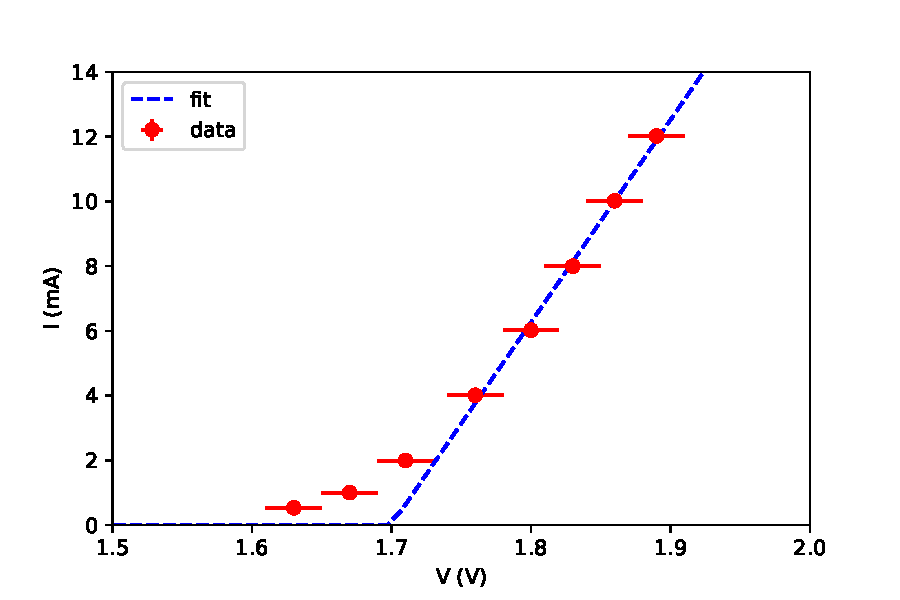
\includegraphics[width=0.45\textwidth]{figs/labs/planck/fit_diode.pdf} &
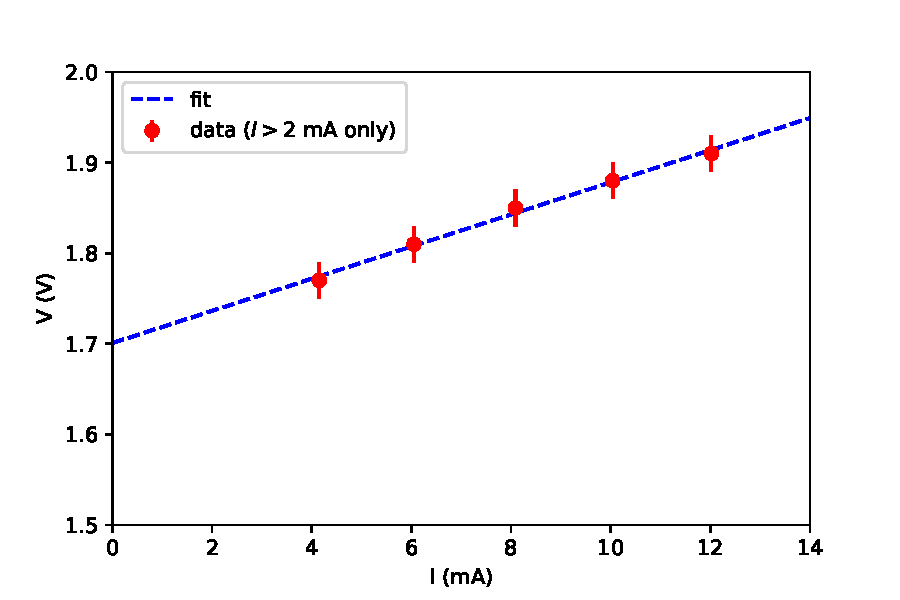
\includegraphics[width=0.45\textwidth]{figs/labs/planck/fit_vi.pdf} \\
(a) & (b) \\
\end{tabular}
\end{center}
\caption{Example fit for red LED.  The (a) real diode response
  departs from the simple linear model for $I \leq 2~\rm mA$, so the
  (b) fit for the linear response is performed for $I > 2~\rm mA$.
  Note that $V_{\rm D}$ is taken as the $y$-axis for the purpose of fit,
  because the voltage uncertainties are the dominant uncertainty in
  the fit.  Notice also that the $0.02~\rm V$ uncertainty reported by
  the DMM specifications appears to be predominantly systematic.}
\label{fig:redfit}
\end{figure}

The example of the V-I response for a red diode is
plotted in Fig~\ref{fig:redfit}a.  Notice that at large values for the
current ($I > 2~\rm mA$) the V-I response is linear, indicating that it
is dominated by internal resistance of the diode.  As lower current
($I \leq 2~\rm mA$) the V-I response is exponential, as expected for a
real diode.  We will fit our simple linear model for the diode
response only in the region where this approximation is valid, for
$I>2~\rm mA$. 

As shown in Fig.~\ref{fig:redfit}b, perform a linear
fit only for the data with $I>2~\rm mA$.

%With the DMM set to the $20~\rm V$ scale, the uncertainty on your
%measured values for $V$ and $I$ is approximately $0.02~\rm V$ and
%$0.02~\rm mA$ respectively.  



\begin{measurement} 
Because the measured voltage range is
less than a volt, but the measured current range is around $10~\rm
mA$, it is the uncertainties on the voltage that dominate the
uncertainty on both the slope and intercept of the linear function in our fit range. Show this is true for your measurement by looking at the percent uncertainties of $I$ and $V_{\rm D}$ that you recorded in your logbook. Record your observation in the logbook.
\end{measurement}


We therefore choose to use $V$ as the $y$-axis and and $I$ as the
$x$-axis for the purposes of fitting, because the $\chi^2$ analysis of
the {\rm curve{\_}fit} function only considers uncertainties in the
$y$-axis.  There are straightforward ways to handle uncertainties in
both $x$ and $y$, but they add complexity which is best avoided if
possible.

\begin{plot} For red LED data, fit the $V$ versus $I$ data to a linear function, and
determine the best fit resistance and activation voltage, and the
uncertainties.  
%Assume the uncertainty on the measured voltages is $0.02~\rm V$ for each data point 
Use uncertainties on the measured voltages
and only consider $I > 2~\rm mA$ in
the fit.  Remember to set {\tt absolute(\_)sigma=True} in your fit so
that the fit uncertainties are based on the absolute uncertainties
without re-scaling. \end{plot}

\begin{plot} 
Repeat this analysis for yellow LED data.
\end{plot}

\begin{plot} 
Repeat this analysis for green LED data.
\end{plot}

\begin{figure}[htbp]
\begin{center}
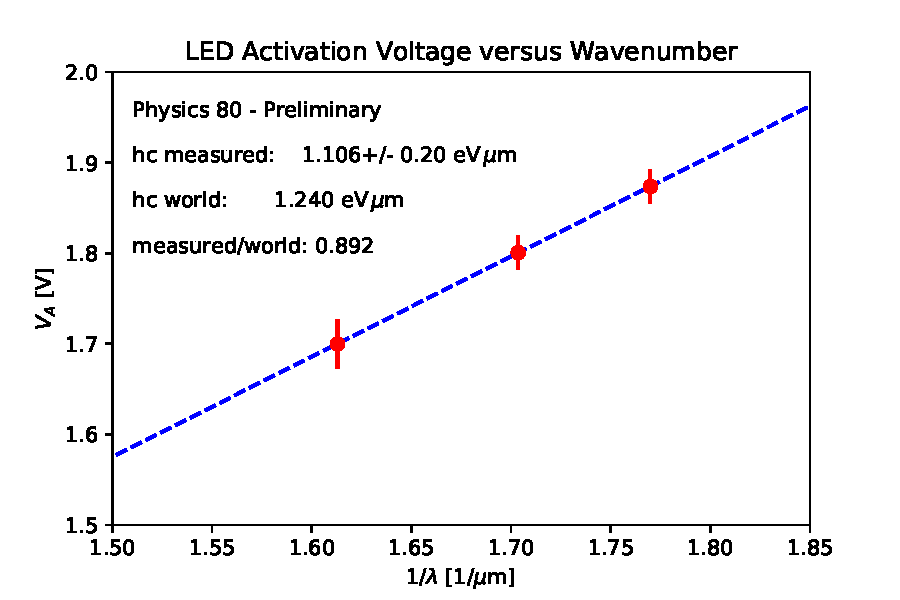
\includegraphics[height=0.3\textheight]{figs/labs/planck/planck.pdf} \\
\end{center}
\caption{Example plot for determination of $hc$.}
\label{fig:planckfit}
\end{figure}

\begin{plot} 
Plot the best-fit $V_A$ of each diode versus $1/\lambda$, and
determine the slope ($hc/e$) and its uncertainty from a linear
fit.  The example plot is shown in Fig.~\ref{fig:planckfit}.
Recall that $1~\rm eV$ is the change in potential energy of one
electron passing through $1~\rm V$ of potential energy, allowing you
to conveniently convert the slope in $\rm V \mu m$ to $\rm eV \mu m$ for
comparison with the established value $hc = 1.240~\rm eV \mu m$.
\end{plot}
\begin{print}
Does your measured value of  $hc$ agree with the known value? Print how many  sigma values your  measured value lies with respect to the known value, as well as your brief comment on this.
\end{print}


\section{Systematic Uncertainties}

In addition to the statistical uncertainties reported by the fit,
their are a number of systematic uncertainties.  For this lab, we'll
consider one obvious source of systematic uncertainty, which arises
from our treatment of the real diode response as a simple linear
function.

To determine the size of this systematic uncertainty, we measure the
effect of this assumption on our measured valued.  One simple way to
estimate this effect is to remove the requirement $I>2~\rm mA$ from
our analysis.  The difference between the measured value for $hc$ as
determined with and without the cut on $I>2~\rm mA$ can be interpreted
as a systematic uncertainty due to our simplistic model.

\begin{print} Repeat your analysis without the requirement $I > 2~\rm mA$ and take
this as the overall systematic uncertainty on your measurement. Print your result in the following form 
\begin{displaymath}
 \textbf{hc}= \textit{your value here} \pm \textit{your value here} \,  ({\rm stat}) \pm\textit{ your value here} \, ({\rm syst})
\end{displaymath}
\end{print}

\noindent
This is a \textbf{sign-off point} for this lab. 












